%!TEX root = ../report.tex
\chapter{Methodology}

In line with the goal of the project to use resource efficient deep learning in terms of inference time and storage memory, the DeepLab v3+ model with MobileNetv2 \cite{DBLP:journals/corr/abs-1801-04381} and Xception \cite{DBLP:journals/corr/Chollet16a} network backbones was chosen. In order to better understand DeepLabv3+, we consider breaking down the architectures of the previous versions of DeepLab leading upto the current version. The different versions of DeepLab are DeepLab \cite{DBLP:journals/corr/ChenPKMY14}, DeepLabv2 \cite{DBLP:journals/corr/ChenPK0Y16}, DeepLabv3 \cite{DBLP:journals/corr/ChenPSA17} and DeepLabv3+ \cite{DBLP:journals/corr/abs-1802-02611}. Also, we review the quantization method considered for this work.

\section{DeepLab}

Fully Convolutional Networks \cite{7298965} were introduced by Long et al. for the task of semantic segmentation. The predictions obtained with the help of this network were coarse and the object boundaries were not sufficiently delineated. In order to overcome these difficulties, the authors of DeepLab proposed the use of atrous convolutions and fully-connected Conditional Random Fields (CRF).

Atrous convolutions, also called as dilated convolutions, is used to gather a better global context with enlarged field-of-view on the feature maps. An atrous rate "r", determines the field-of-view of an atrous convolution. With increase in atrous rate, a greater region of a feature map is convolved over. This leads to gathering of more global context. However, it is worth noting that there is no increase in the number of parameters in the convolution filter. Only the convolved region in the input feature map changes. When the atrous rate is 1, standard convolution is performed. The Figure \ref{Fig:atconv} illustrates atrous convolution. 

	\begin{figure}
		\centering
		\begin{subfigure}{.27\textwidth}
			\centering
			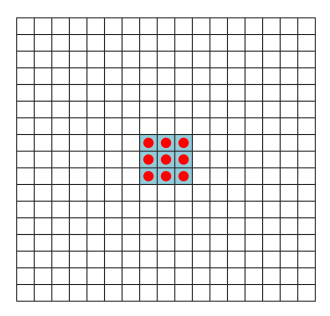
\includegraphics[width=1\linewidth]{images/r_1}
			\caption{Atrous rate = 1}
		\end{subfigure}
		\begin{subfigure}{.27\textwidth}
			\centering
			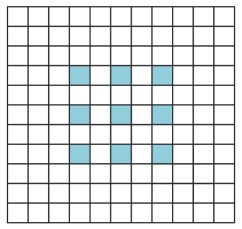
\includegraphics[width=1\linewidth]{images/r_2}
			\caption{Atrous rate = 2}
		\end{subfigure}
		\begin{subfigure}{.27\textwidth}
			\centering
			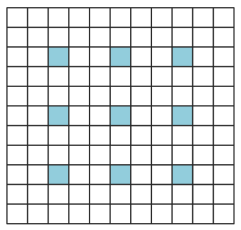
\includegraphics[width=1\linewidth]{images/r_3}
			\caption{Atrous rate = 3}
		\end{subfigure}
		\caption{Illustration of 3$\times$3 atrous convolution with three different atrous rates \cite{DBLP:journals/corr/Garcia-GarciaOO17}. The blue squares denote the parameters of the convolution filter. The white grid space represents the input feature map. The field-of-view grows with increase in atrous rate but not the number of parameters.}
		\label{Fig:atconv}
	\end{figure}
	
Fully-connected Conditional Random Fields (CRF), is used to post process the prediction of the segmentation network used in DeepLab, to improve object delineation. Every pixel in the output feature map is connected to every other pixel resulting in pairwise terms. In each pairwise term, based on color and position, the similarity between pixels is determined and a class is assigned for the pixels.


\section{DeepLabv2}

% Source: http://www.davidtvs.com/exploring-semantic-segmentation-dnn/
In DeepLabv2, Atrous Spatial Pyramid Pooling (ASPP) was used in addition to the existing architecture. The authors also use deeper ResNet network to improve accuracy.

Atrous Spatial Pyramid Pooling, is used to create multiscale feature representations. Atrous convolutions with different atrous rates are applied to the same feature map. The resulting feature maps from each atrous convolution is processed in separate branches in a similar fashion as in DeepLabv1 by using two 1$\times$1 convolutions. Each of the branches are then fused together to obtain multiscale information. The ASPP module is illustrated in Figure \ref{Fig:aspp}. The difference between the ASPP modules of DeepLabv1 and DeepLabv2 is illustrated in Figure \ref{Fig:v1vsv2}.

	\begin{figure}
		\centering
		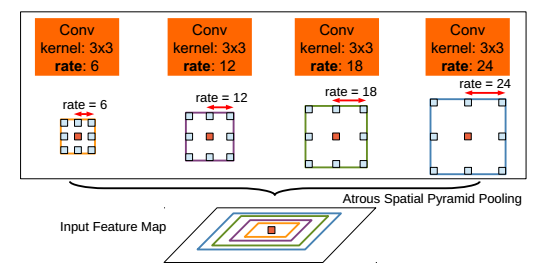
\includegraphics[width=0.6\linewidth]{images/aspp}
		\caption{Illustration of Atrous Spatial Pyramid Pooling (ASPP). Atrous convolutions with 4 different rates convolve on the same input feature map. The field-of-view of each atrous rate is shown using different colors \cite{DBLP:journals/corr/ChenPK0Y16}.}
		\label{Fig:aspp}
	\end{figure}
	
	\begin{figure}
		\begin{subfigure}{.5\textwidth}
			\centering
			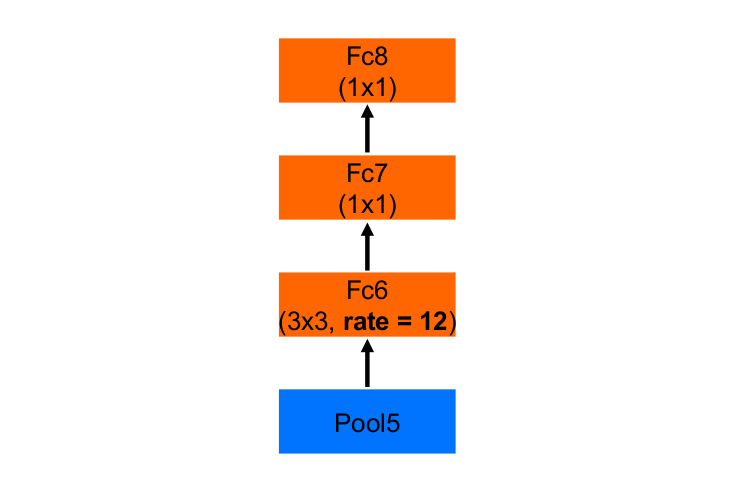
\includegraphics[width=1.03\linewidth]{images/v1_largeFOV}
			\caption{Large field-of-view in DeepLabv1}
		\end{subfigure}
		\begin{subfigure}{.5\textwidth}
			\centering
			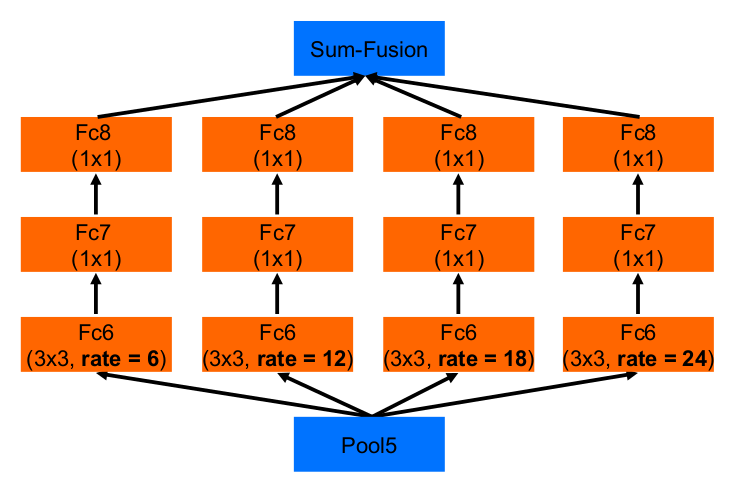
\includegraphics[width=1\linewidth]{images/v2_aspp}
			\caption{ASPP in DeepLabv2}
		\end{subfigure}
		\caption{Illustration of the difference in architecture between DeepLabv1 and DeepLabv2 \cite{DBLP:journals/corr/ChenPK0Y16}.}
		\label{Fig:v1vsv2}
	\end{figure}
	
\section{DeepLabv3}
In this version of DeepLab, the contributions include improvements to the context module, and the use of batch normalization. Batch Normalization is applied to every layer in the context module and the parameters of the batch normalization layers are trained.

The authors experiment with two different modules to handle context one being a cascade module and the other being an improved version of ASPP module. The cascade module is formed by repeating the last block from ResNet and replacing convolutions with atrous convolutions. The authors report that performing this repetition upto three times improves performance. 	The cascade module is illustrated in Figure \ref{Fig:contextmodulea}. The ASPP module used in DeepLabv3 is similar to the one used in DeepLabv2. However, the difference now is that the ASPP module uses five branches. The first four branches perform 1$\times$1 convolution, and three 3$\times$3 convolutions with atrous rates 6, 12 and 18. The 5th branch provides image level features by performing global average pooling on the last feature maps of the model. The resulting channels are concatenated and projected to a different channel space using 1$\times$1 convolution.

	\begin{figure}
		\begin{subfigure}{1\textwidth}
			\centering
			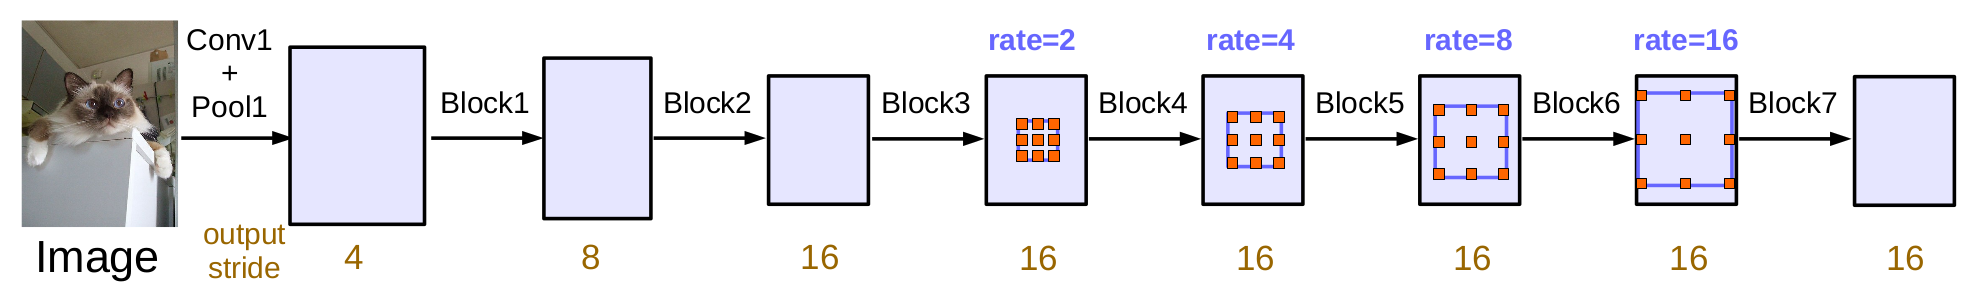
\includegraphics[width=1\linewidth]{images/cascade_module}
			\caption{cascade module in DeepLabv3}
			\label{Fig:contextmodulea}
		\end{subfigure}
		\begin{subfigure}{1\textwidth}
			\centering
			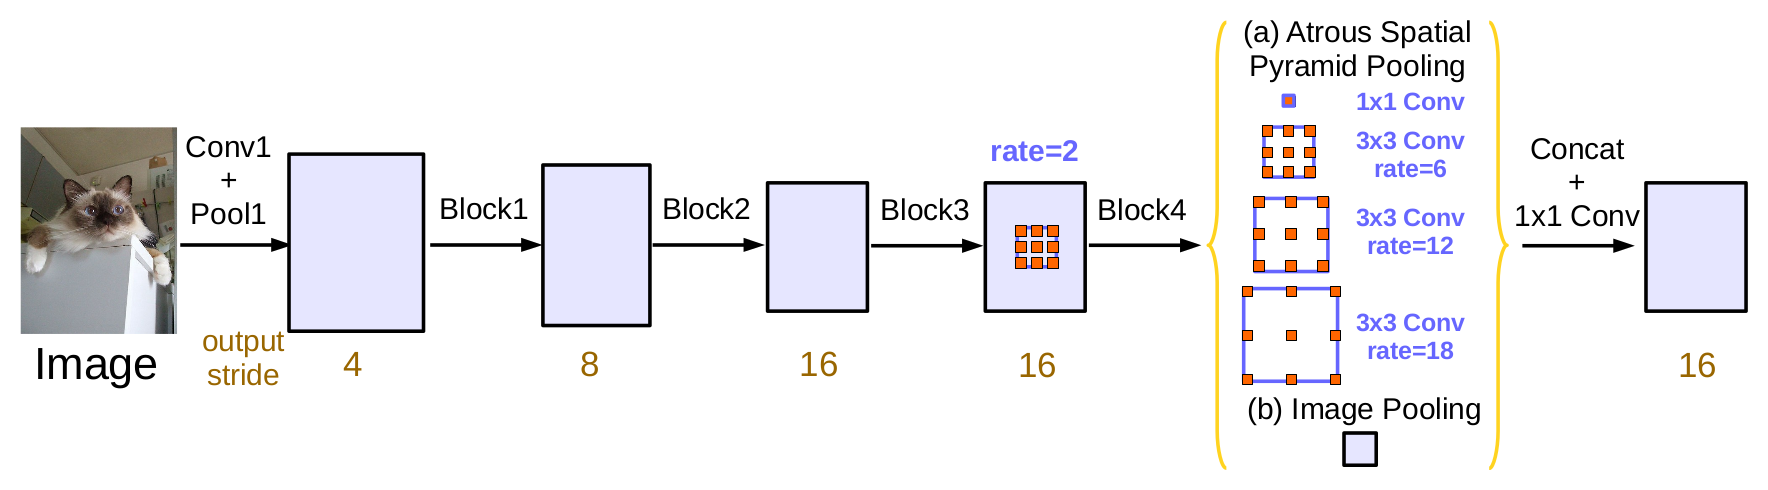
\includegraphics[width=1\linewidth]{images/aspp_module}
			\caption{ASPP module in DeepLabv3}
			\label{Fig:contextmoduleb}
		\end{subfigure}
		\caption{Illustration of two different context modules used in deepLabv3 \cite{DBLP:journals/corr/ChenPSA17}.}
		\label{Fig:contextmodule}
	\end{figure}

\section{DeepLabv3+}

DeepLabv3+ is designed to combine the ability of ASPP module which can capture rich context information and the ability of encoder-decoder networks which can produce sharp object boundary delineation. Xception, MobileNetv2 and ResNet-101 are used as encoders out of which this project only considers Xception and MobileNetv2 for their resource efficiency. The major differences in DeepLabv3+ is the use of a decoder, the use of atrous separable convolutions in both the encoder and decoder and the adaption of MobileNetv2 and Xception as network backbones (encoders).

The authors call the ratio of input resolution to the output resolution before global average pooling as the output stride. DeepLabv3 is designed to have an output stride of 16. To bring the prediction to the original image resolution, the final features are upsampled by a factor of 16 using bilinear interpolation. This is considered by the authors as a naive decoder module. Instead of this naive approach, the authors propose the use of a better decoder module. The final encoder features are first upsampled by a factor of 4, and are concatenated with the low level features from the encoder with same dimensions. The number of channels in the low level features are first reduced using a 1$\times$1 convolution. A 3$\times$3 convolution convolves over this concatenated features to refine the features and is later followed by an upsampling of 4 to lead to the final prediction. The architecture of DeepLabv3+ is depicted in Figure \ref{Fig:deepLabv4}.

	\begin{figure}
		\centering
		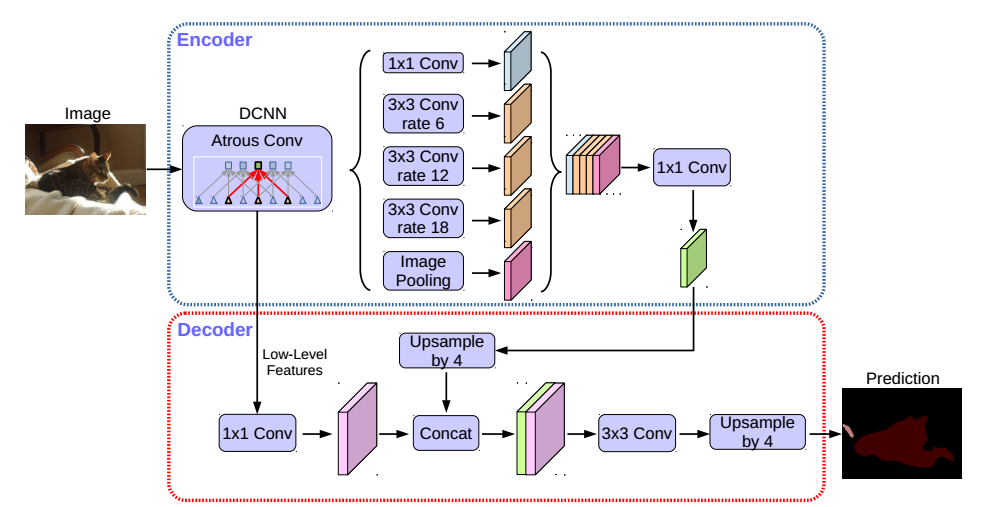
\includegraphics[width=1\linewidth]{images/deepLabv4}
		\caption{An illustration of DeepLabv3+ architecture. The encoder extracts features at different scales and the decoder refines object boundary delineation \cite{DBLP:journals/corr/abs-1802-02611}.}
		\label{Fig:deepLabv4}
	\end{figure}

The MobileNetv2 and Xception encoders make use of depthwise separable convolutions to improve resource efficiency. Section \ref{section:mn} and Section \ref{section:xcep} provide details regarding MobileNetv2 and Xception architectures respectively. In DeepLabv3+, the authors use atrous convolution instead of depthwise convolution in depthwise seperable convolution. The authors call this type of convolution as atrous separable convolution and state that these convolutions can be used to extract feature maps at arbitrary resolution. The authors use a modified version of the Xception architecture as depicted in Figure \ref{Fig:deepLabv4_xcep} as one of the network backbones.

	\begin{figure}
		\centering
		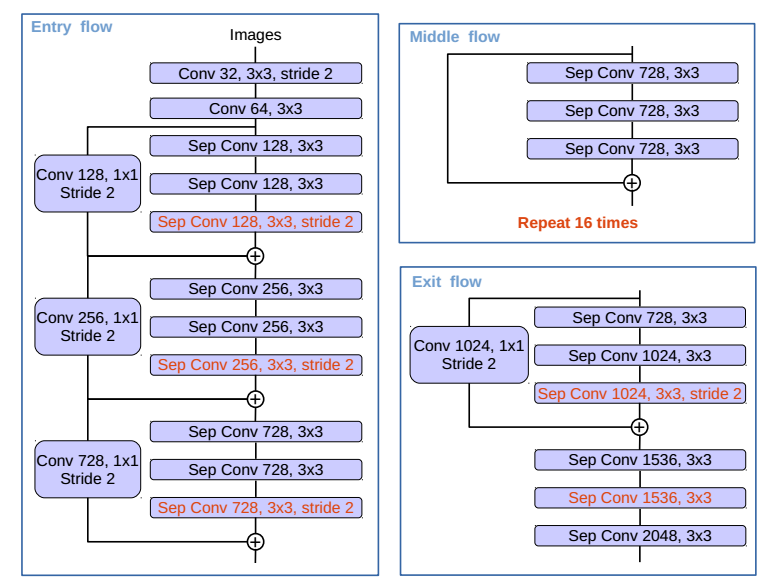
\includegraphics[width=.8\linewidth]{images/deepLabv4_xcep}
		\caption{Modified Xception architecture used as encoder in DeepLabv3+. The max pooling operations in the original Xception architecture are replaced with depthwise separable convolutions. Batch normalization and ReLU activation is applied after each 3$\times$3 depthwise convolution \cite{DBLP:journals/corr/abs-1802-02611}.}
		\label{Fig:deepLabv4_xcep}
	\end{figure}

\section{MobileNetv2}
\label{section:mn}

% to cite: https://towardsdatascience.com/mobilenetv2-inverted-residuals-and-linear-bottlenecks-8a4362f4ffd5

% mobileNetv2 building block: https://ai.googleblog.com/2018/04/mobilenetv2-next-generation-of-on.html 

% depthwise : https://eli.thegreenplace.net/2018/depthwise-separable-convolutions-for-machine-learning/

The MobileNetv2 architecture is designed to work on mobile and embedded devices where computational resources are limited. The authors state that their main contribution is the use of a novel layer module called the inverted residual with linear bottleneck. 

Depthwise separable convolutions, known for its efficiency, is used in this work. Standard convolution layers are replaced with two layers where the first layer performs depthwise convolution and the second layer performs pointwise convolution. A depthwise convolution layer uses a single fiter per input channel to perform convolution. The pointwise convolution layer consists of 1$\times$1 convolutions which perform weighted linear combination on the input channels and projects them to a new channel space. This factorization of standard convolution layer into two separate depthwise and pointwise layers leads to roughly $k^2$ times reduction in computation cost where k is the kernel size of the convolutional filter. Figure \ref{Fig:depthwise} illustrates depthwise convolution. In this case, pointwise convolution performs dimensionality reduction as the number of output channels is less than number of input channels. However, if more than 3 pointwise convolutions are used, dimensionality of output channels can be increased.

	\begin{figure}
		\centering
		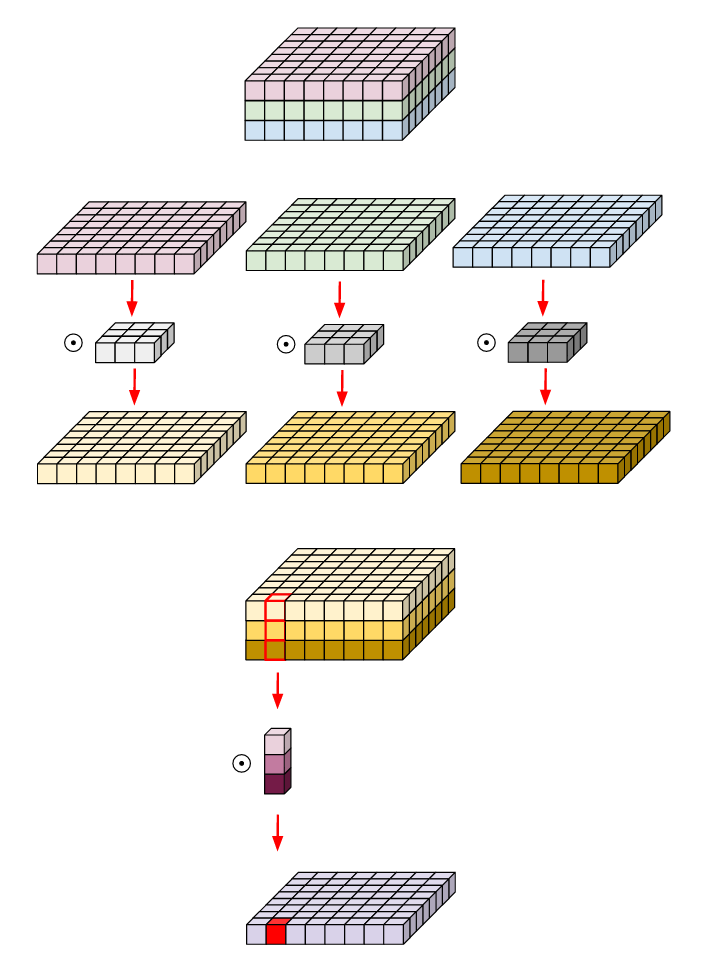
\includegraphics[width=.5\linewidth]{images/depthwise}
		\caption{An illustration of depthwise separable convolution with 3 input channels and 1 output channel. The first row shows the three input channels. The next three rows illustrate three separate 3$\times$3 convolutions convolving over one of the input channels. The fifth row shows the resulting feature maps of the three convolutions being stacked upon each other. Rows 2 to 5 together is the depthwise convolution. The sixth row shows a pointwise convolution convolving over the output of depthwise convolution to get the final output channel \cite{depthwise}.}
		\label{Fig:depthwise}
	\end{figure}

In the original residual block \cite{DBLP:journals/corr/HeZRS15}, first a 1$\times$1 convolution is used to reduce the number of channels. On this reduced number of channels 3$\times$3 standard convolution is done which is followed by a 1$\times$1 convolution which now expands the feature maps to have the same number of channels as the input to the block. A skip connection is then introduced through which the input channels is added to the output channels of the residual block. The skip connection provides a layer with access to earlier activations and also helps prevent the vanishing gradients problem. 

The authors of MobileNetv2 propose the use of inverted residual block which takes advantage of depthwise seperable convolutions. This block consists of a narrow bottleneck layer followed by a 1$\times$1 convolution which performs expansion of number of channels. Depthwise convolution is performed on the expanded input channels followed by a pointwise convolution which brings down the number of channels to create the next bottleneck layer. A skip connection is then added between the input bottleneck and the output bottleneck. The original and inverted residual blocks are depicted in Figure \ref{Fig:residual}. The authors use linear activation in the bottleneck layers and hypothesize that it is better than non-linear activation.

	\begin{figure}
		\begin{subfigure}{.5\textwidth}
			\centering
			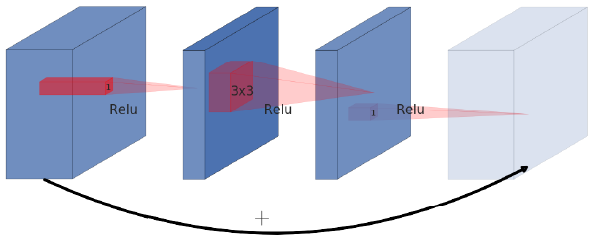
\includegraphics[width=.8\linewidth]{images/residual}
			\caption{Residual block}
		\end{subfigure}
		\begin{subfigure}{.5\textwidth}
			\centering
			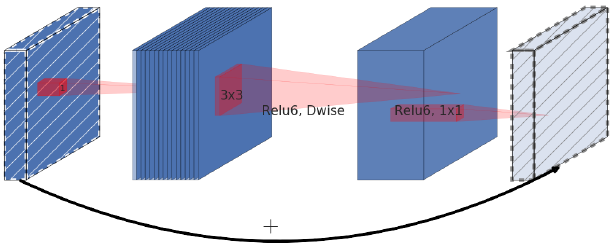
\includegraphics[width=.8\linewidth]{images/inverted_residual}
			\caption{Inverted residual block}
		\end{subfigure}
		\caption{Illustration of the original residual block and the inverted residual block used by MobileNetv2 \cite{DBLP:journals/corr/abs-1801-04381}.}
		\label{Fig:residual}
	\end{figure}

This hypothesis is based on the notion that the ReLU activation layer used, leads to information loss due to loss of values less than 0. However, loss of too much information due to the induced nonlinearity by the activation can be prevented by the use of linear activation in the bottleneck layer. The authors show that a linear activation is empirically better than a non linear activation in the bottleneck layer.

The inverted residual block has less number of parameters than the residual block and with linear bottleneck is shown to achieve state-of-the-art performance. The inverted residual block is visualized in the architecture of MobileNetv2 in Figure \ref{Fig:mobileNetv2bb}.

	\begin{figure}
		\centering
		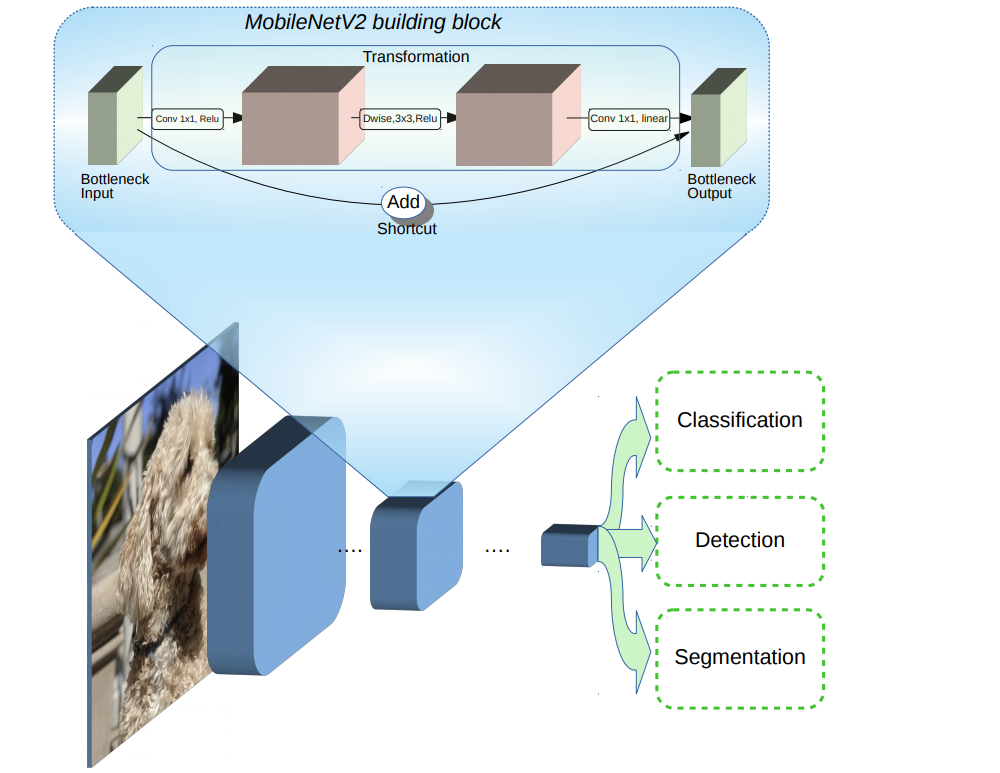
\includegraphics[width=.7\linewidth]{images/mobileNetv2_bb}
		\caption{The building block of MobileNetv2. The compressed representation obtained could be used for tasks such as image classification, object detection and semantic segmentation \cite{mnbb}.}
		\label{Fig:mobileNetv2bb}
	\end{figure}

\section{Xception}
\label{section:xcep}

The Xception architecture is derived based on two hypothesis made by the authors. One hypothesis is based on the inception architecture and the other is a stronger version of the inception hypothesis. Standard convolution layers has 3D convolution kernals which maps both spatial correlations and cross-channel correlations at the same time. Here spatial correlations is obtained by mapping correlations across the height and the width of every channel separately. Cross-channel correlations is obtained at every spatial location across the height and width of the channels, from each of the channels in the input. 

In the Inception architecture, an inception module consists of 4 branches operating on the same input feature maps. The different branches of the inceptionv3 module is shown in Figure \ref{Fig:xceptiona}. In the second branch with 1$\times$1 convolution followed by a 3$\times$3 convolution, the 1$\times$1 convolution calculates the cross-channel correlation between the input channels and performs dimensionality reduction by reducing the number of input channels. Next, the 3$\times$3 convolution is a standard convolution which looks for both spatial and cross-channel correlations in this reduced input channel space. Since this inception module has lead to state-of-the-art classification results, the authors hypothesize that the cross-channel correlations and spacial correlations are decoupled and can be mapped separately. This is evidently based on the fact that the inception module partially handles spatial and cross-channel correlations in a decoupled fashion by using a 1$\times$1 convolution followed by a 3$\times$3 convolution. 

	\begin{figure}
		\begin{subfigure}{.5\textwidth}
			\centering
			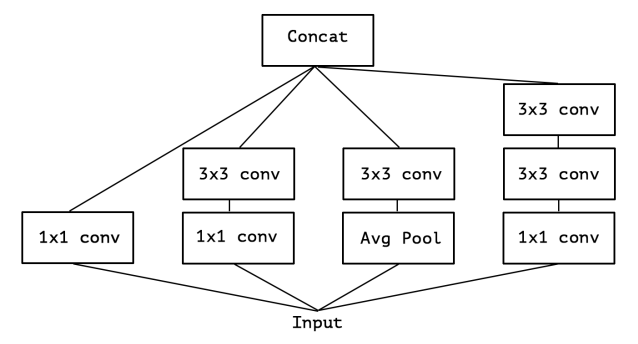
\includegraphics[width=1\linewidth]{images/inception_v3}
			\caption{Inceptionv3 module}
			\label{Fig:xceptiona}
		\end{subfigure}
		\begin{subfigure}{.5\textwidth}
			\centering
			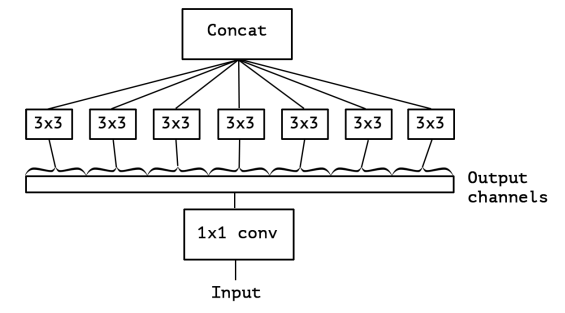
\includegraphics[width=1\linewidth]{images/extreme_inception}
			\caption{Extreme version of inception module}
			\label{Fig:xceptionb}
		\end{subfigure}
		\caption{Illustration of the inception v3 module and an extreme version of the inception module. In the extreme version, each of the 3$\times$3 convolution operates on a single output channel of 1$\times$1 convolution \cite{DBLP:journals/corr/Chollet16a}.}
		\label{Fig:xception}
	\end{figure}

Based on this hypothesis, the authors propose that the two correlations can be mapped completely independent of each other leading to a stronger hypothesis. An illustration of this stronger hypothesis can be seen in Figure \ref{Fig:xceptionb}. The Xception network is based on this stronger hypothesis and is named "Xception" as the architecture is an extreme version of inception. The complete decoupling of the two correlations, could be obtained using depthwise separable convolution, as evidently, this type of convolution first performs depthwise convoltion which handles the spatial correlation and then performs pointwise convolution which handles cross-channel correlation.

The authors show that the use of depthwise separable convolutions enables the Xception architecture to achieve a marginally better top-1 and top-5 accuracy than the Inception V3 architecture despite the fact that Xception has less number of parameters. This experimental observation suggests that Xception is resource efficient and is also powerful in terms of "learning capacity".

%\section{Pruning}

%A trained Deep Convolutional Neural Network (DCNN) might have learnable parameters which are redundant in terms of its effect on the test time accuracy. Pruning aims to identify such redundant learnable parameters and remove them, thereby leading to compression of the DCNN. State-of-the-art methods provide different criteria to determine this redundancy which are discussed in "State of the Art" section.

%Most of the literature identified for this work concerning pruning, do not provide open source implementations of their work. 

%\textbf{[In progress..might be dropped]}

\section{Quantization}

This work makes use of the quantization method available in tensorflow source repository \footnote{\url{https://github.com/tensorflow/tensorflow/blob/master/tensorflow/tools/quantization/quantize_graph.py}}. "eightbit" mode is used to obtain a quantized tensorflow inference graph. The blog in \cite{quant_blog} provides a description of this quantization procedure.

Neural networks, in general, learn features which are robust to noise in the input image such as changes in illumination. As an extension, it is possible to speculate that loss in precision induced by low-precision calculations is ignored by a neural network as another source of noise. High precision calculation, though necessary to handle gradient propagation during training, might not be necessary during inference. Quantizing a neural network calculations to low-precision could therefore be a way to reduce computation cost without much loss in accuracy in order to facilitate usage on an embedded device. More specifically, quantizing calculations to eight bit calculations would make  a neural network faster and reduce storage requirements on embedded devices. 

	\begin{figure}
		\begin{subfigure}{.4\textwidth}
			\centering
			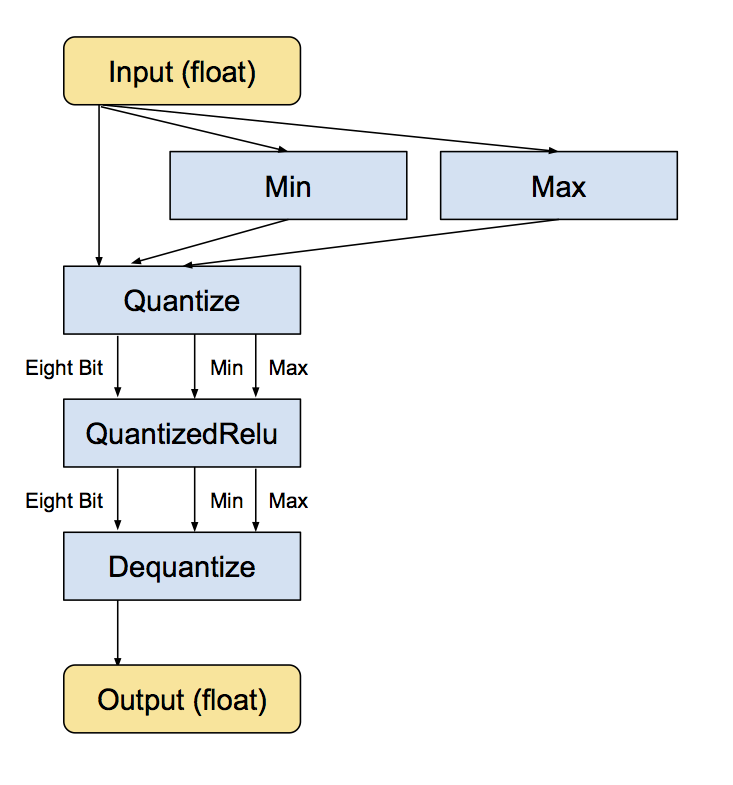
\includegraphics[width=1\linewidth]{images/quantization1}
			\caption{}
			\label{Fig:quantizationb}
		\end{subfigure}
		\begin{subfigure}{.6\textwidth}
			\centering
			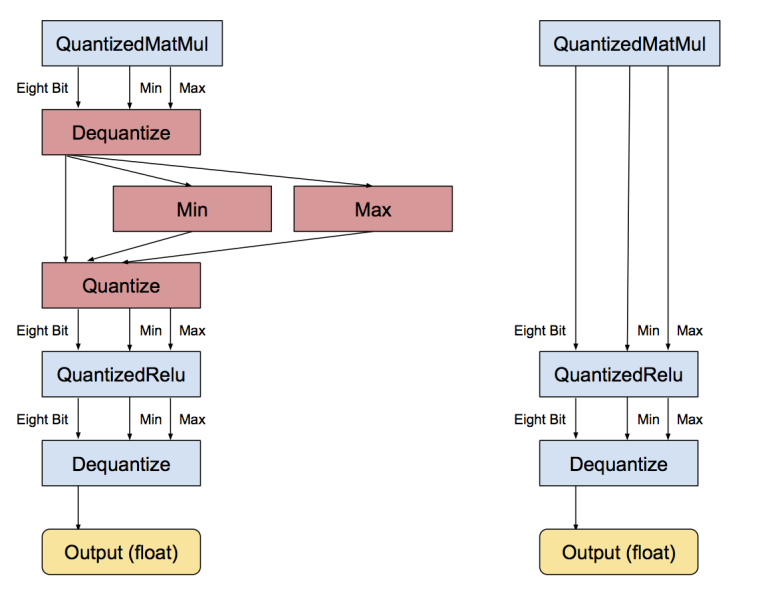
\includegraphics[width=1\linewidth]{images/quantization2}
			\caption{}
			\label{Fig:quantizationa}
		\end{subfigure}
		\caption{ This figure shows illustrations of the quantization procedure available in tensorflow source. (a) Replacing an operation with a subgraph which performs qantization, corresponding quantized operation and dequantization. (b) The figure on the left shows a redundant subgraph (indicated in red) in between two quantized operations and the figure on the right shows the graph obtained after removing the redundant subgraph \cite{quant_blog}.}
		\label{Fig:quantization}
	\end{figure}

The quantization algorithm replaces common operations such as convolution, activation functions and pooling operations with equivalent quantized operations. The input data is converted from float to eight bit precision by adding a subgraph as illustrated in Figure \ref{Fig:quantizationa}. The algorithm also identifies sequences of quantized operations and removes subgraphs which perform redundant conversion as illustrated in Figure \ref{Fig:quantizationb}. The overall maximum and minimum possible values of weights and activation tensors are representated by the lowest and highest quantized values respectively which is 0 and 255 for eight bit. The rest of the values of the tensors are then represented within the range of eight bits. This format of quantization brings certain advantages such as the ability to represent arbitrary ranges and negative numbers, and the linear spread of values facilitates multiplication. The minimum and maximum values are determined by the "QuantizeDownAndShrinkRange" operator which analyzes and rescales the tensor to eight bit in a manner that the range of eight bit values is used effectively.